\documentclass[journal]{IEEEtran}

\usepackage{amsmath,amssymb,amsfonts}
\usepackage{graphicx}
\usepackage{booktabs}
\usepackage{tabularx}
\usepackage{multirow}
\usepackage{cite}
\usepackage{url}
\usepackage{xcolor}
\usepackage{tikz}
\usetikzlibrary{arrows.meta,positioning,fit,calc}
\usepackage{algorithm}
\usepackage{algorithmic}
\usepackage{balance}
\usepackage{subcaption}

\begin{document}

\title{Confidence-Gated Multi-Agent Fall Detection: Retrieval-Augmented Reasoning and Cost-Sensitive Response on Wearable IMU Data}

\author{%
\IEEEauthorblockN{Anonymous Authors}
\IEEEauthorblockA{%
\textit{Anonymous Institution}\\
Email: anonymous@institution.edu}
}

\maketitle

\begin{abstract}
Wearable inertial fall detectors can look strong on average accuracy and still fail where it matters: near-fall activities that sit between clear falls and clear activities of daily living (ADLs), and operating points that ignore the asymmetry between missed falls and false alarms. We study a complementary question to detector design---given a fixed Tier-1 CNN--LSTM--Attention model in the spirit of Bhatti \textit{et al.}, can a decision-time wrapper improve the safety operating point? We propose a \emph{Risk-Calibrated Dual-Process} (RCDP) stack: a dual-threshold confidence gate routes easy windows on-device (System~1), while ambiguous windows escalate to biomechanical evidence serialization, MiniLM $k$-NN case retrieval, local LLM chain-of-thought reasoning, and a cost-sensitive Action Agent (System~2). On a SisFall \emph{ambiguous stress benchmark} (D18/D19 near-falls, $n{=}300$/fold), Tier-1 mean F1 is $0.713$ and rises to $0.896$ with the full stack ($\Delta\text{F1}{=}+0.183$, $\Delta\text{Recall}{=}+0.208$, $\approx 84\%$ cost-per-window reduction). Under subject-independent five-fold evaluation on the main protocol ($n{=}1000$/fold), F1 improves from $0.759{\pm}0.014$ to $0.887{\pm}0.029$ and recall from $0.759{\pm}0.022$ to $0.977{\pm}0.037$, with normalized response cost cut by roughly $83\%$. Binary KFall transfer is confirmatory stability (F1 $0.987{\rightarrow}0.990$), not a headline F1 jump. Paired ambiguous-case comparisons show local Mistral far above a heuristic reasoner (mean F1 $0.972$ vs.\ $0.034$). We also report honest escalation rates, split-conformal gate audits, IMU orientation/sampling robustness, and a negative actor--critic study. Gains are versus the \emph{same} Tier-1 checkpoints under a locked protocol; we do not claim to displace published multi-phase KFall detector tables.
\end{abstract}

\begin{IEEEkeywords}
Fall detection, wearable IMU, confidence gating, selective prediction, retrieval-augmented reasoning, large language models, cost-sensitive learning, SisFall, conformal prediction.
\end{IEEEkeywords}

\section{Introduction}
\label{sec:intro}

Falls remain a leading cause of injury among older adults, and wearable IMUs are an attractive sensing modality for continuous monitoring at home~\cite{iglesias2019wearable,nurek2020fallsurvey,khan2017review,sisfall2017}. Deep detectors have narrowed the gap to strong benchmark accuracy~\cite{ren2021survey}, yet three deployment gaps persist. Near-fall motions---stumbles, abrupt sits, compensatory recoveries---produce windows that a forced binary classifier must label even when the kinematics are genuinely ambiguous~\cite{aziz2016fall}. Softmax scores are often poorly calibrated for deferral~\cite{guo2017calibration,geifman2017selective,el2010foundations}. And a fall/ADL bit is not a response policy: emergency dispatch, caregiver notify, monitor, and log have unequal clinical and operational costs, especially when false negatives dominate risk~\cite{elkan2001foundations}.

Bhatti \textit{et al.}~\cite{bhatti2025beyond} present a capable hybrid CNN--LSTM--Attention detector for multi-phase fall analysis (``Beyond Falls''). That line of work is primarily about \emph{detection}. We ask a different question: \emph{holding the detector fixed, can an agentic wrapper improve the safety operating point---raising recall and lowering expected response cost---while producing structured rationales on the hard cases?}

Our answer is a Risk-Calibrated Dual-Process (RCDP) pipeline. System~1 is a fast edge reflex ($\approx 7$\,ms): a fixed Tier-1 detector plus a cost-calibrated dual-threshold gate. System~2 is deliberative triage for the ambiguous band: serialize biomechanical evidence $\Sigma(w)$, retrieve similar past cases with MiniLM embeddings~\cite{minilm2020,lewis2020rag}, run local LLM chain-of-thought reasoning~\cite{wei2022cot,yao2023react,ollama,mistral2023}, and emit a graded action under asymmetric cost
\begin{equation}
\mathcal{R}_\beta = \beta\cdot\mathrm{FN}+\mathrm{FP},\qquad \beta=10.
\label{eq:risk}
\end{equation}
Primary evaluation uses SisFall~\cite{sisfall2017} with subject-independent five-fold splits, forced D18/D19 near-fall coverage, a homogeneous $n{=}1000$ test budget per fold, an ambiguous stress benchmark ($n{=}300$), multi-seed Ollama sweeps, latency profiles, and completed binary KFall external validation~\cite{kfall2021}.

\paragraph{Contributions.}
\begin{itemize}
\item An end-to-end agentic architecture---gate, evidence, retrieval, LLM CoT, action---wrapped around a Bhatti-style Tier-1 backbone without updating its weights at inference (Fig.~\ref{fig:arch}, Alg.~\ref{alg:rcdp}).
\item A locked evaluation protocol (splits, calibration, cost, near-fall metrics) supporting cumulative ablations \texttt{tier1\_only}$\rightarrow$\texttt{gate\_only}$\rightarrow$\texttt{gate\_knn}$\rightarrow$\texttt{gate\_llm}$\rightarrow$\texttt{gate\_knn\_llm}.
\item SisFall evidence that the full stack improves F1/recall and normalized cost on every main-protocol fold, with lead gains on the ambiguous stress benchmark (Tier-1 F1 $0.713$ vs.\ stack $0.896$, $\Delta\text{F1}{=}+0.183$).
\item Paired LLM backend comparisons, budget/latency analyses, binary KFall stability checks, split-conformal gate audits, IMU robustness, and an explicit negative study of label-flip actor--critic vetoing.
\item Honest positioning: numerical gains are versus the \emph{same} Tier-1 checkpoints under our protocol; we do not claim to supersede Bhatti's original multi-phase KFall tables.
\end{itemize}

\section{Related Work}
\label{sec:related}

\subsection{Wearable Fall Detection}
Threshold rules~\cite{bourke2007threshold} and classical learners gave way to CNN, LSTM, TCN, and Transformer variants on SisFall~\cite{sisfall2017}, KFall~\cite{kfall2021}, UP-Fall~\cite{martinez2019upfall}, and UniMiB SHAR~\cite{micucci2017unimib}. Surveys stress the free-living trade-off between sensitivity and nuisance alarms~\cite{iglesias2019wearable,khan2017review,ren2021survey}. Bhatti \textit{et al.}~\cite{bhatti2025beyond} combine CNN, LSTM, and attention for pre-/transition-/post-fall phases on KFall. We reuse that architectural motif as Tier-1 and invest the novelty in decision-time agents rather than another backbone bake-off as the sole claim.

\subsection{Uncertainty, Selective Prediction, and Conformal Methods}
Networks are frequently miscalibrated~\cite{guo2017calibration,platt1999probabilistic}. Selective classification and abstention~\cite{el2010foundations,geifman2017selective} motivate routing uncertain inputs to stronger decision makers. Split conformal prediction provides finite-sample set-valued predictions with coverage control under exchangeability~\cite{vovk2005algorithmic,angelopoulos2023gentle}. Learning under label-dependent costs goes back at least to Elkan's foundations~\cite{elkan2001foundations}; for binary decisions the Bayes threshold under $\mathcal{R}_\beta$ is $\tau^*=1/(\beta{+}1)$. Our primary gate is cost-calibrated dual-threshold deferral; we additionally audit a split-conformal gate as a complementary selective mechanism (Sec.~\ref{sec:conformal}).

\subsection{Retrieval-Augmented and Agentic LLM Reasoning}
RAG~\cite{lewis2020rag} and compact encoders such as MiniLM~\cite{minilm2020} support case-based prompting. Chain-of-thought~\cite{wei2022cot} and reason--act loops~\cite{yao2023react} improve structured decisions. Local runtimes~\cite{ollama,mistral2023,qwen2024} keep CoT offline. We apply these ideas to IMU-derived evidence strings---not open-domain text---and close the loop with a cost-sensitive Action Agent. Related sensing-agent systems debate without explicit FN-heavy clinical cost or near-fall stress protocols; we keep those constraints front and center.

\section{Method}
\label{sec:method}

Fig.~\ref{fig:arch} and Alg.~\ref{alg:rcdp} summarize the pipeline.

\begin{figure*}[!t]
\centering
% TikZ architecture figure for agentic fall detection pipeline
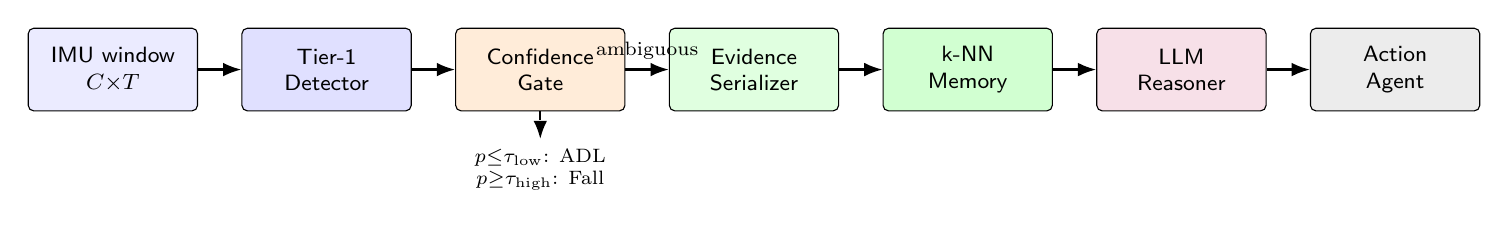
\begin{tikzpicture}[
  font=\footnotesize,
  box/.style={draw, rounded corners=2pt, align=center, inner sep=4pt, minimum height=1.05cm, minimum width=2.15cm},
  arr/.style={-{Latex}, thick},
  every node/.style={font=\footnotesize\sffamily}
]
\node[box, fill=blue!8] (imu) {IMU window\\$C{\times}T$};
\node[box, fill=blue!12, right=0.55cm of imu] (tier1) {Tier-1\\Detector};
\node[box, fill=orange!15, right=0.55cm of tier1] (gate) {Confidence\\Gate};
\node[box, fill=green!12, right=0.55cm of gate] (ev) {Evidence\\Serializer};
\node[box, fill=green!18, right=0.55cm of ev] (knn) {k-NN\\Memory};
\node[box, fill=purple!12, right=0.55cm of knn] (llm) {LLM\\Reasoner};
\node[box, fill=gray!15, right=0.55cm of llm] (act) {Action\\Agent};

\draw[arr] (imu) -- (tier1);
\draw[arr] (tier1) -- (gate);
\draw[arr] (gate) -- node[above, font=\scriptsize] {ambiguous} (ev);
\draw[arr] (ev) -- (knn);
\draw[arr] (knn) -- (llm);
\draw[arr] (llm) -- (act);

\node[below=0.35cm of gate, font=\scriptsize, align=center] (direct) {$p{\le}\tau_{\mathrm{low}}$: ADL\\$p{\ge}\tau_{\mathrm{high}}$: Fall};
\draw[arr, dashed] (gate.south) -- (direct.north);
\end{tikzpicture}

\caption{Confidence-gated multi-agent fall detection. High- and low-confidence windows are resolved by the Tier-1 detector; ambiguous windows escalate to evidence serialization, $k$-NN retrieval, LLM reasoning, and a cost-sensitive Action Agent.}
\label{fig:arch}
\end{figure*}

\begin{algorithm}[!t]
\caption{RCDP inference for one IMU window}
\label{alg:rcdp}
\begin{algorithmic}[1]
\REQUIRE Window $\mathbf{x}\in\mathbb{R}^{C\times T}$; Tier-1 $f_\theta$; gate $(\tau_{\mathrm{low}},\tau_{\mathrm{high}})$; memory $\mathcal{M}$; LLM $\mathcal{L}$; Action Agent $\mathcal{A}$
\STATE Compute logits and embedding: $(\boldsymbol{\ell},\mathbf{e})\leftarrow f_\theta(\mathbf{x})$
\STATE $p\leftarrow \mathrm{softmax}(\boldsymbol{\ell})_1$ \COMMENT{fall probability}
\IF{$p\le\tau_{\mathrm{low}}$}
  \STATE $\hat{y}\leftarrow\mathrm{ADL}$; $a\leftarrow\texttt{log}$
\ELSIF{$p\ge\tau_{\mathrm{high}}$}
  \STATE $\hat{y}\leftarrow\mathrm{Fall}$; $a\leftarrow\texttt{alarm}$
\ELSE
  \STATE Serialize evidence $\Sigma(\mathbf{x})$; retrieve $N_k\leftarrow\mathrm{Top}\text{-}k(\mathcal{M},\Sigma)$
  \STATE $(\hat{y},r)\leftarrow\mathcal{L}(\Sigma(\mathbf{x}),N_k)$ \COMMENT{JSON label + rationale}
  \STATE $a\leftarrow\mathcal{A}(\hat{y},r,\Sigma(\mathbf{x}))$ \COMMENT{graded action}
\ENDIF
\STATE \textbf{return} $(\hat{y},a,p)$
\end{algorithmic}
\end{algorithm}


\subsection{Tier-1 Detector}
Let $\mathbf{x}\in\mathbb{R}^{C\times T}$ denote an IMU window ($C{=}6$, $T{=}90$ on SisFall). A backbone $f_\theta$ maps $\mathbf{x}$ to logits $\boldsymbol{\ell}\in\mathbb{R}^{2}$ and an embedding $\mathbf{e}$. The fall probability is
\begin{equation}
p = \Pr(y{=}1\mid\mathbf{x}) = \frac{e^{\ell_1}}{e^{\ell_0}+e^{\ell_1}}.
\label{eq:pfall}
\end{equation}
The primary backbone is CNN--LSTM--Attention following Bhatti~\textit{et al.}~\cite{bhatti2025beyond}. We also train a detector zoo (CNN1D, LSTM, CNN--LSTM, TCN, ModernTCN~\cite{iglesias2023modern}, TSMixer~\cite{tsmixer2023}, PatchTST~\cite{patchtst2023}, Transformer~\cite{vaswani2017attention}) under the same protocol for context (Table~\ref{tab:backbone}), but all agentic tables freeze \texttt{cnn\_lstm\_attn}.

\subsection{Confidence Gate}
A dual-threshold gate with calibrated $(\tau_{\mathrm{low}},\tau_{\mathrm{high}})$ routes windows:
\begin{equation}
\mathrm{route}(p)=
\begin{cases}
\mathrm{ADL}, & p \le \tau_{\mathrm{low}},\\
\mathrm{Fall}, & p \ge \tau_{\mathrm{high}},\\
\mathrm{Ambiguous}, & \text{otherwise.}
\end{cases}
\label{eq:gate}
\end{equation}
Thresholds are fit on subject-held-out calibration windows by grid search that scores only confident (edge) decisions under FN/FP costs and a mild deferral penalty (Alg.~\ref{alg:gate}). Mode \texttt{tier1\_only} collapses escalation to a point decision at $0.5$.

\begin{algorithm}[!t]
\caption{Cost-calibrated dual-threshold gate and split-conformal audit}
\label{alg:gate}
\begin{algorithmic}[1]
\REQUIRE Calibration set $\{(p_i,y_i)\}_{i=1}^{n}$; costs $(\beta_{\mathrm{FN}},\beta_{\mathrm{FP}})$; conformal level $\alpha$
\STATE \textbf{Cost gate:} grid-search $(\tau_{\mathrm{low}},\tau_{\mathrm{high}})$ minimizing $\beta_{\mathrm{FN}}\!\cdot\!\mathrm{FN}_{\mathrm{edge}}+\beta_{\mathrm{FP}}\!\cdot\!\mathrm{FP}_{\mathrm{edge}}+\lambda\cdot\mathrm{deferral}$ on confident decisions only
\STATE \textbf{Conformal:} scores $s_i\leftarrow 1-p_i$ if $y_i{=}1$ else $1-(1-p_i)$
\STATE $\hat{q}\leftarrow$ $(1-\alpha)$-quantile of $\{s_i\}$ with finite-sample correction $\lceil(n{+}1)(1{-}\alpha)\rceil/n$
\STATE For test $p$: prediction set $C(p)=\{c:\,1{-}\hat{p}(c)\le\hat{q}\}$
\STATE If $|C|{=}1$ route at the edge; if $|C|{=}2$ escalate (ambiguous)
\STATE Audit edge FN rate on held-out confident decisions; report escalation rate
\STATE \textbf{return} $(\tau_{\mathrm{low}},\tau_{\mathrm{high}},\hat{q})$
\end{algorithmic}
\end{algorithm}


\subsection{Evidence Serializer}
For escalated windows we compute kinematic descriptors---free-fall duration proxies, impact magnitude, post-impact stillness, tilt change, peak gyroscope---and serialize them into a natural-language evidence string $\Sigma(\mathbf{x})$ consumed by retrieval and the LLM.

\subsection{Retrieval Memory}
A $k$-NN memory stores MiniLM~\cite{minilm2020} embeddings of evidence text with labels and features. At escalation we retrieve $k{=}5$ neighbors by cosine similarity as few-shot context~\cite{lewis2020rag}:
\begin{equation}
\mathrm{sim}(\mathbf{u},\mathbf{v})=\frac{\mathbf{u}^\top\mathbf{v}}{\|\mathbf{u}\|_2\|\mathbf{v}\|_2}.
\label{eq:cosine}
\end{equation}

\subsection{LLM Reasoner}
A local reasoner (Ollama/Mistral by default; heuristic and Qwen2.5 for paired comparisons) consumes $\Sigma(\mathbf{x})$ and neighbors and returns a JSON object with predicted label and rationale~\cite{wei2022cot,mistral2023,qwen2024,ollama}. Production full-stack rows use Ollama with Mistral.

\subsection{Action Agent and Clinical Cost}
The Action Agent maps severity cues to simulated actions $\{\texttt{emergency},\texttt{notify},\texttt{monitor},\texttt{log}\}$. Aggregate evaluation cost follows~\eqref{eq:risk} with $\beta{=}10$; we report cost per $1000$ windows so equal-budget folds are comparable. Under~\eqref{eq:risk} the offline Bayes threshold for a single hard classifier (no deferral) is
\begin{equation}
\tau^{*}=\frac{1}{\beta+1}=\frac{1}{11}\approx 0.091,
\label{eq:tau_star}
\end{equation}
which we evaluate as a no-escalation partition fallback (Table~\ref{tab:partitionfallback}).

\subsection{System Modes}
Ablations instantiate cumulative agents:
\texttt{tier1\_only}, \texttt{gate\_only}, \texttt{gate\_knn}, \texttt{gate\_llm}, and \texttt{gate\_knn\_llm} (full stack). The ladder isolates whether gains require retrieval, language-model reasoning, or both.

\subsection{Deployment Workflow}
\label{sec:deployment}
Fig.~\ref{fig:deployment} sketches the dual-process deployment view. System~1 runs on-device in milliseconds. Ambiguous windows escalate to System~2 during the post-impact immobility window (tens of seconds), where latency budgets are less severe than free-fall impact protection. Table~\ref{tab:escalation} reports honest escalation rates by protocol---about $47\%$ on the main SisFall protocol, $59\%$ on the ambiguous stress set, and $\approx 1.1\%$ on binary KFall.

\begin{figure*}[!t]
\centering
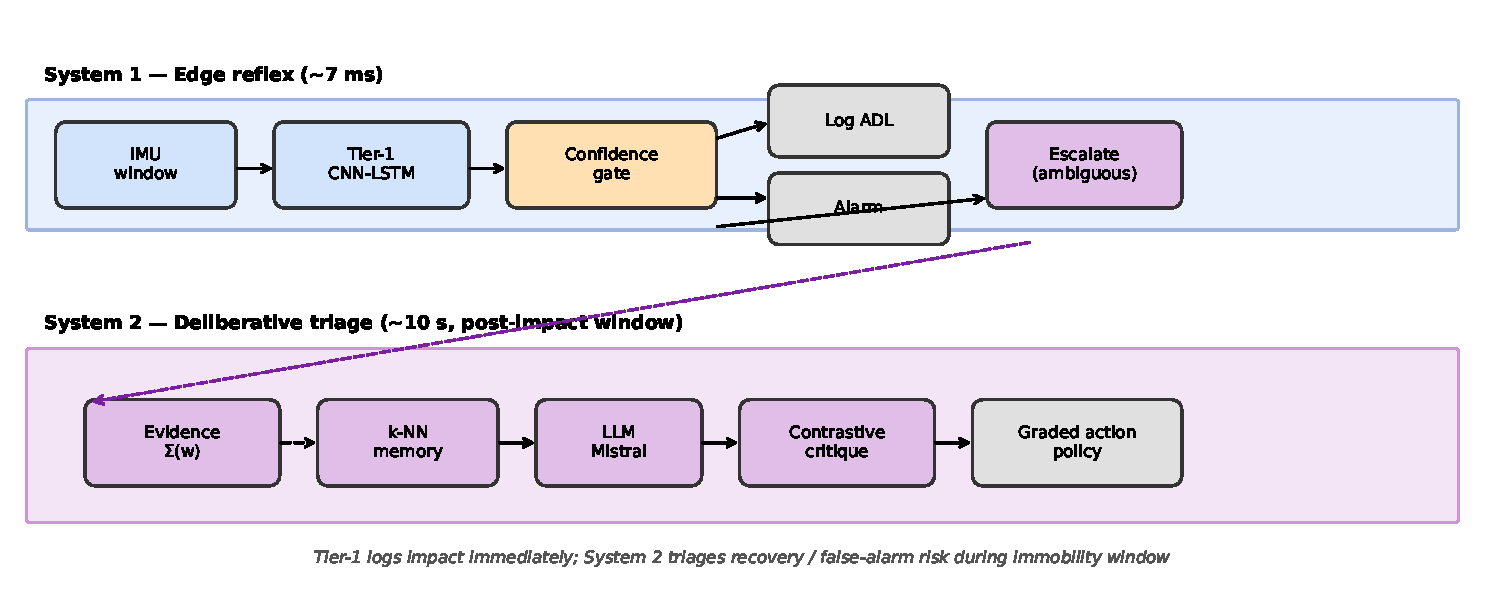
\includegraphics[width=\linewidth]{figures/deployment_architecture.pdf}
\caption{RCDP deployment workflow: System~1 edge reflex (milliseconds) versus System~2 deliberative triage (seconds) on escalated ambiguous windows.}
\label{fig:deployment}
\end{figure*}

\begin{table}[!t]
\centering
\caption{System~2 escalation duty cycle by evaluation protocol (honest reporting). High rates on the ambiguous stress benchmark reflect deliberate near-fall stress; KFall external transfer invokes deliberation on $\approx$1\% of windows.}
\label{tab:escalation}
\begin{tabular}{lcc}
\toprule
Protocol & $n$/fold & Escalation rate \\
\midrule
SisFall main (5-fold mean) & 1000 & 0.47 ($\pm$0.08) \\
SisFall ambiguous stress & 300 & 0.59 \\
KFall external (5-fold mean) & 1000 & 0.011 \\
\bottomrule
\end{tabular}
\end{table}


\subsection{Clinical Cost Framing and Grounding}
\label{sec:clinical}
Risk~\eqref{eq:risk} and threshold~\eqref{eq:tau_star} make the FN/FP asymmetry explicit (Table~\ref{tab:betacost}). To check that LLM rationales cite telemetry rather than invented severity, we measure kinematic faithfulness $\mathcal{G}_{\mathrm{faith}}$: the fraction of rationales that mention primitives from $\Sigma(\mathbf{x})$ (Table~\ref{tab:grounding}). Contrastive critique raises mean $\mathcal{G}_{\mathrm{faith}}$ from $0.436$ to $0.843$ and reduces graded action cost by about $45\%$.

\begin{table}[!t]
\centering
\caption{Asymmetric clinical cost sensitivity across penalty ratio $\beta=c_{\mathrm{FN}}/c_{\mathrm{FP}}\in\{5,10,20\}$ (cost $=\beta\cdot\mathrm{FN}+\mathrm{FP}$, per 1000 windows). Bayes optimal threshold $\tau^*=1/(\beta+1)$ motivates asymmetric escalation.}
\label{tab:betacost}
\begin{tabular}{lcccc}
\toprule
$\beta$ & $\tau^*$ & Mode & Mean cost/1000 & $\Delta$ vs Tier-1 \\
\midrule
5 & 0.167 & tier1\_only & 628 & --- \\
5 & 0.167 & \textbf{gate\_knn\_llm} & \textbf{149} & \textbf{-479} \\
\addlinespace
10 & 0.091 & tier1\_only & 1151 & --- \\
10 & 0.091 & \textbf{gate\_knn\_llm} & \textbf{200} & \textbf{-951} \\
\addlinespace
20 & 0.048 & tier1\_only & 2197 & --- \\
20 & 0.048 & \textbf{gate\_knn\_llm} & \textbf{302} & \textbf{-1895} \\
\bottomrule
\end{tabular}
\end{table}

\begin{table}[!t]
\centering
\caption{Kinematic faithfulness $\mathcal{G}_{\mathrm{faith}}$ (rationale grounding rate): fraction of LLM rationales citing biomechanical evidence $\Sigma(w)$ (impact $g$, stillness, tilt). Contrastive critique nearly doubles grounding with $\approx$45\% graded action cost reduction.}
\label{tab:grounding}
\begin{tabular}{ccccc}
\toprule
Fold & Base $\mathcal{G}_{\mathrm{faith}}$ & +Contrastive & Graded cost base & Graded cost +Critique \\
\midrule
0 & 0.430 & 0.851 & 544 & 268 \\
1 & 0.340 & 0.749 & 901 & 599 \\
2 & 0.471 & 0.871 & 535 & 261 \\
3 & 0.482 & 0.874 & 428 & 216 \\
4 & 0.459 & 0.868 & 537 & 274 \\
\midrule
Mean & 0.436 & \textbf{0.843} & 589 & \textbf{324} \\
\bottomrule
\end{tabular}
\end{table}


\section{Experimental Setup}
\label{sec:setup}

\subsection{Dataset and Splits}
SisFall~\cite{sisfall2017} provides six-channel IMU windows (window length $90$, hop $10$) from $38$ subjects after processing ($\approx 1.55{\times}10^{6}$ windows). Subject-independent five-fold splits hold out subjects; within each training fold a subject-held-out validation fraction tunes training and gate calibration. Near-fall codes D18 (stumble) and D19 (sudden sit) are required and forced into capped test slices (minimum $80$ windows per code). Main tables use a homogeneous stratified budget of $n{=}1000$ per fold for LLM-tractable escalation; $n{=}4000$ archives support budget sensitivity and detailed ablations. The ambiguous stress benchmark uses $n{=}300$ per fold ($100$ D18/D19 + $100$ falls + $100$ clear ADLs).

\subsection{Training and Agentic Protocol}
Training uses class \texttt{pos\_weight}, mixup, and cost-sensitive decision thresholds. The global seed for primary tables is $42$; Fold~0 multi-seed sweeps use $\{42,43,44\}$ with Ollama/Mistral. Primary agentic backend is local Ollama/Mistral. Locked settings live in \texttt{configs/paper\_protocol.yaml}.

\subsection{Metrics and Statistics}
We report F1, recall/sensitivity, specificity, near-fall false-alarm rate on D18/D19, escalated-subset F1, escalation rate, normalized response cost, and latency (Tier-1 ms vs.\ escalated-path seconds). Significance uses paired bootstrap $95\%$ confidence intervals (BCa when $n{\ge}3$) on fold-wise deltas; Wilcoxon signed-rank $p$-values are reported for completeness. With unanimous signs at $n{=}5$, Wilcoxon $p$ floors at $0.0625$; bootstrap CIs that exclude zero are the primary uncertainty claim.

\subsection{External Validation (KFall)}
KFall~\cite{kfall2021} is the corpus emphasized in Beyond Falls. We evaluate binary Fall/ADL windows under the same cost/gate protocol (five subject-independent folds). We additionally report a Fold~0 36-class Tier-1 context run that is \emph{not} a claim against published multi-class leaderboards.

\section{Results}
\label{sec:results}

Table~\ref{tab:positioning} situates the work: Bhatti~\textit{et al.} optimize multi-phase detection; we optimize a decision system around a detector.

\begin{table*}[!t]
\centering
\caption{Positioning relative to Bhatti \textit{et al.} (base detector paper).}
\label{tab:positioning}
\begin{tabular}{lll}
\toprule
Aspect & Bhatti \textit{et al.}~2025~\cite{bhatti2025beyond} & This work \\
\midrule
Primary task & Multi-phase fall/ADL classification & Detection + uncertainty + explanation + response \\
Backbone & CNN--LSTM--Attention & Same primary backbone + modern zoo \\
Uncertainty & Softmax confidence only & Dual-threshold confidence gate ($\tau_{\mathrm{low}},\tau_{\mathrm{high}}$) \\
Explainability & Attention weights & Structured biomechanical evidence + CoT JSON \\
Case memory & None & Retrieval-augmented $k$-NN memory \\
Response policy & None & Cost-sensitive Action Agent \\
Primary dataset in original paper & KFall (multi-class) & SisFall binary + near-fall ADLs (D18/D19) \\
Fair baseline in our tables & --- & \texttt{tier1\_only} (same checkpoint/folds) \\
\bottomrule
\end{tabular}
\end{table*}


\subsection{Ambiguous Stress Benchmark (Lead Result)}
\label{sec:ambiguous}
D18/D19 near-falls are where softmax detectors most often fail silently. On the dedicated ambiguous stress set (Table~\ref{tab:ambiguoussisfall}), Tier-1 mean F1 is $0.713$ while \texttt{gate\_knn\_llm} reaches $0.896$ ($\Delta\text{F1}{=}+0.183$, $\Delta\text{Recall}{=}+0.208$, cost/window $0.90{\rightarrow}0.15$). Escalation is high ($\approx 59\%$) by construction: the benchmark is a stress test, not a free-living duty-cycle claim.

\begin{table*}[!t]
\centering
\caption{SisFall \emph{ambiguous stress benchmark} ($n{=}300$/fold: 100 D18/D19 near-fall + 100 fall + 100 clear ADL). Tier-1 F1 collapses on near-fall activities; the full stack recovers performance. Cost is clinical safety cost ($10\cdot\mathrm{FN}+\mathrm{FP}$) per window; Esc.\ is System~2 escalation rate.}
\label{tab:ambiguoussisfall}
\begin{tabular}{c r ccc ccc cc}
\toprule
Fold & $n$ & \multicolumn{3}{c}{Tier-1} & \multicolumn{3}{c}{gate\_knn\_llm} & $\Delta$F1 & Esc. \\
\cmidrule(lr){3-5}\cmidrule(lr){6-8}
 & & F1 & Rec. & Cost/win & F1 & Rec. & Cost/win & & rate \\
\midrule
0 & 300 & 0.696 & 0.790 & 0.86 & 0.868 & 0.990 & 0.13 & +0.172 & 0.59 \\
1 & 300 & 0.738 & 0.790 & 0.82 & 0.894 & 0.930 & 0.28 & +0.156 & 0.52 \\
2 & 300 & 0.682 & 0.750 & 0.98 & 0.892 & 0.990 & 0.11 & +0.210 & 0.63 \\
3 & 300 & 0.714 & 0.760 & 0.92 & 0.902 & 0.970 & 0.16 & +0.189 & 0.61 \\
4 & 300 & 0.735 & 0.750 & 0.93 & 0.922 & 1.000 & 0.06 & +0.186 & 0.62 \\
\midrule
Mean & 300 & 0.713 & 0.768 & 0.90 & \textbf{0.896} & \textbf{0.976} & \textbf{0.15} & \textbf{+0.183} & 0.59 \\
\bottomrule
\end{tabular}
\end{table*}


\subsection{Main Comparison versus Tier-1}
On the main $n{=}1000$ protocol, Table~\ref{tab:perfold} shows F1 gains on every fold ($+0.114$ to $+0.164$). Five-fold means (Table~\ref{tab:meanstd}) move F1 from $0.759$ to $0.887$, recall from $0.759$ to $0.977$, and cost/1000 from $1151$ to $200$ ($\approx 83\%$ reduction). Table~\ref{tab:stats} reports BCa bootstrap CIs that exclude zero with $5/5$ fold sign consistency. Fig.~\ref{fig:costf1} visualizes the paired pattern.

\begin{figure}[!t]
\centering
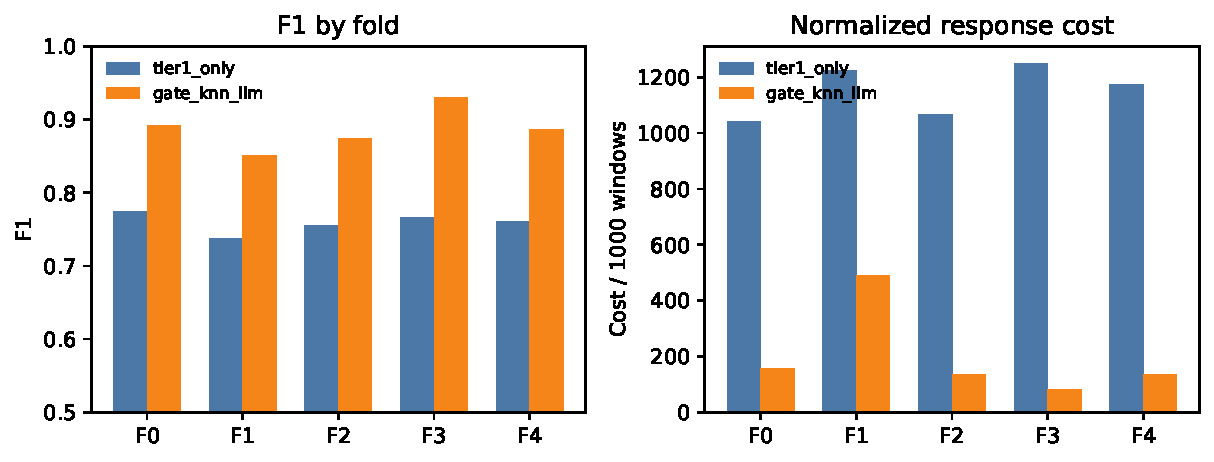
\includegraphics[width=\linewidth]{figures/cost_f1_per_fold.pdf}
\caption{Per-fold F1 and normalized response cost for \texttt{tier1\_only} versus \texttt{gate\_knn\_llm} under the homogeneous $n{=}1000$ protocol.}
\label{fig:costf1}
\end{figure}

\begin{table*}[!t]
\centering
\caption{Per-fold comparison of Tier-1 (\texttt{tier1\_only}) vs.\ full agentic stack (\texttt{gate\_knn\_llm}) under the homogeneous protocol ($n{=}1000$ stratified windows/fold with forced D18/D19). Cost is normalized per 1000 windows.}
\label{tab:perfold}
\begin{tabular}{c r ccc ccc c}
\toprule
Fold & $n$ & \multicolumn{3}{c}{Tier-1} & \multicolumn{3}{c}{gate\_knn\_llm} & $\Delta$F1 \\
\cmidrule(lr){3-5}\cmidrule(lr){6-8}
 & & F1 & Rec. & Cost/1k & F1 & Rec. & Cost/1k & \\
\midrule
0 & 1000 & 0.774 & 0.781 & 1042 & 0.892 & 0.986 & 156 & +0.119 \\
1 & 1000 & 0.737 & 0.748 & 1223 & 0.851 & 0.911 & 490 & +0.114 \\
2 & 1000 & 0.755 & 0.783 & 1066 & 0.874 & 0.998 & 134 & +0.119 \\
3 & 1000 & 0.766 & 0.732 & 1248 & 0.930 & 0.995 & 83 & +0.164 \\
4 & 1000 & 0.760 & 0.749 & 1175 & 0.887 & 0.993 & 136 & +0.126 \\
\bottomrule
\end{tabular}
\end{table*}

\begin{table}[!t]
\centering
\caption{Five-fold mean$\pm$std on SisFall (homogeneous $n{=}1000$). Paired deltas are \texttt{gate\_knn\_llm}$-$\texttt{tier1\_only}. With five folds, Wilcoxon $p{=}0.0625$ is at the discrete minimum for a complete sign agreement; we therefore emphasize bootstrap 95\% CIs.}
\label{tab:meanstd}
\begin{tabular}{lccc}
\toprule
Mode & F1 & Recall & Cost / 1000 \\
\midrule
tier1\_only & 0.759$\pm$0.014 & 0.759$\pm$0.022 & 1151$\pm$93 \\
\textbf{gate\_knn\_llm} & \textbf{0.887$\pm$0.029} & \textbf{0.977$\pm$0.037} & \textbf{200$\pm$164} \\
\midrule
\multicolumn{4}{l}{\textit{Paired $\Delta$ (stack $-$ Tier-1)}} \\
Metric & Mean $\Delta$ & Bootstrap 95\% CI & Wilcoxon $p$ \\
\midrule
F1 & +0.132 & [0.119, 0.144] & 0.0625 \\
Recall & +0.213 & [0.182, 0.238] & 0.0625 \\
Cost/1000 & -936.000 & [-1064.000, -829.447] & 0.0625 \\
\bottomrule
\end{tabular}
\end{table}

\begin{table}[!t]
\centering
\caption{Paired statistics for \texttt{gate\_knn\_llm}$-$\texttt{tier1\_only} across five subject-independent folds ($n{=}5$). Sign column reports folds with improvement (F1/recall$\uparrow$, cost$\downarrow$). With unanimous signs, Wilcoxon $p$ floors at $0.0625$; bootstrap 95\% CIs (BCa when $n{\ge}3$) are primary.}
\label{tab:stats}
\begin{tabular}{lcccc}
\toprule
Metric & Mean $\Delta$ & Bootstrap 95\% CI & Sign & Wilcoxon $p$ \\
\midrule
F1 & +0.132 & [0.119, 0.144] (bca) & 5/5 & 0.0625 \\
Recall & +0.213 & [0.182, 0.238] (bca) & 5/5 & 0.0625 \\
Cost/1000 & -936 & [-1064, -829] (bca) & 5/5 & 0.0625 \\
\bottomrule
\end{tabular}
\end{table}

% Per-fold directional consistency:
% F1 5/5, Recall 5/5, Cost 5/5


\subsection{Ablations}
On Fold~0 with $n{=}4000$ (Table~\ref{tab:ablation}, Fig.~\ref{fig:ablation}), \texttt{gate\_only} matches Tier-1 aggregate F1, \texttt{gate\_knn} alone does not unlock large gains, and \texttt{gate\_llm} without retrieval can inflate near-fall false alarms. The full stack reaches F1 $0.907$, recall $0.993$, and escalated F1 $0.952$ at substantially lower cost. Retrieval and LLM reasoning are complementary. Homogeneous five-fold ablation means appear in Table~\ref{tab:ablationmean}.

\begin{figure}[!t]
\centering
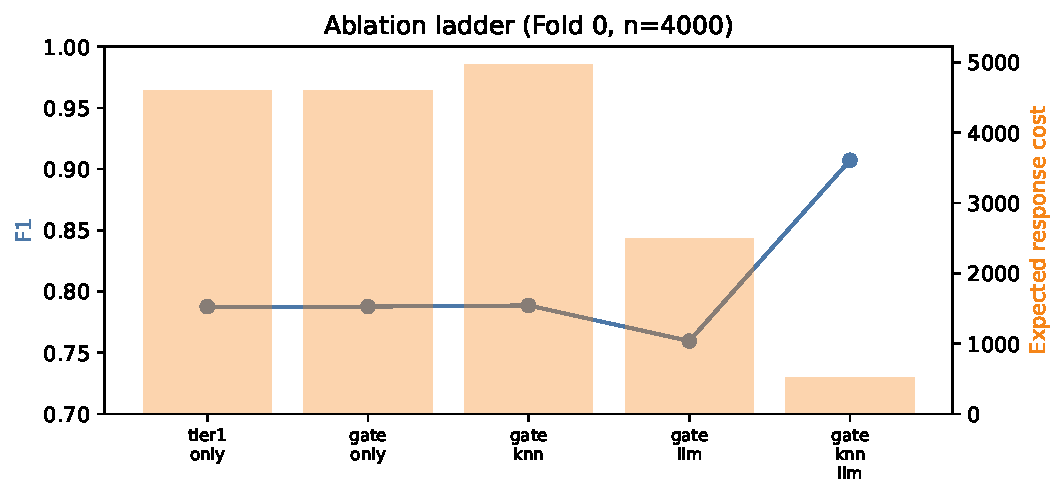
\includegraphics[width=\linewidth]{figures/ablation_ladder.pdf}
\caption{Ablation ladder on Fold~0 ($n{=}4000$ archive): F1 (left axis) and expected response cost (right axis).}
\label{fig:ablation}
\end{figure}

\begin{table}[!t]
\centering
\caption{Ablation ladder on Fold~0 under the full evaluation budget ($n{=}4000$). Gate or $k$-NN alone does not yield the headline gain; the full stack (\texttt{gate\_knn\_llm}) is required.}
\label{tab:ablation}
\begin{tabular}{lccccc}
\toprule
Mode & F1 & Recall & Cost & Near-fall FAR & Esc.\ F1 \\
\midrule
tier1\_only & 0.788 & 0.787 & 4596 & 0.219 & 0.000 \\
gate\_only & 0.788 & 0.787 & 4596 & 0.219 & 0.175 \\
gate\_knn & 0.789 & 0.764 & 4972 & 0.188 & 0.026 \\
gate\_llm & 0.760 & 0.924 & 2491 & 0.625 & 0.445 \\
\textbf{gate\_knn\_llm} & \textbf{0.907} & \textbf{0.993} & \textbf{516} & \textbf{0.212} & \textbf{0.952} \\
\bottomrule
\end{tabular}
\end{table}

\begin{table}[!t]
\centering
\caption{Five-fold mean$\pm$std ablation under the homogeneous $n{=}1000$ protocol.}
\label{tab:ablationmean}
\begin{tabular}{lccc}
\toprule
Mode & F1 & Recall & Cost/1000 \\
\midrule
tier1\_only & 0.759$\pm$0.014 & 0.759$\pm$0.022 & 1151$\pm$93 \\
gate\_only & 0.759$\pm$0.014 & 0.759$\pm$0.022 & 1151$\pm$93 \\
gate\_knn & 0.753$\pm$0.012 & 0.723$\pm$0.032 & 1286$\pm$133 \\
gate\_llm & 0.702$\pm$0.021 & 0.895$\pm$0.027 & 740$\pm$105 \\
\textbf{gate\_knn\_llm} & \textbf{0.887$\pm$0.029} & \textbf{0.977$\pm$0.037} & \textbf{200$\pm$164} \\
\bottomrule
\end{tabular}
\end{table}


\subsection{LLM Backends on Ambiguous Cases}
Table~\ref{tab:llm} and Fig.~\ref{fig:llm} compare reasoners on shared ambiguous IDs. Heuristic mean F1 is near floor ($0.034$), Mistral reaches $0.972$, and Qwen2.5 reaches $0.823$. Escalation without competent language-model reasoning does not explain the recovery.

\begin{figure}[!t]
\centering
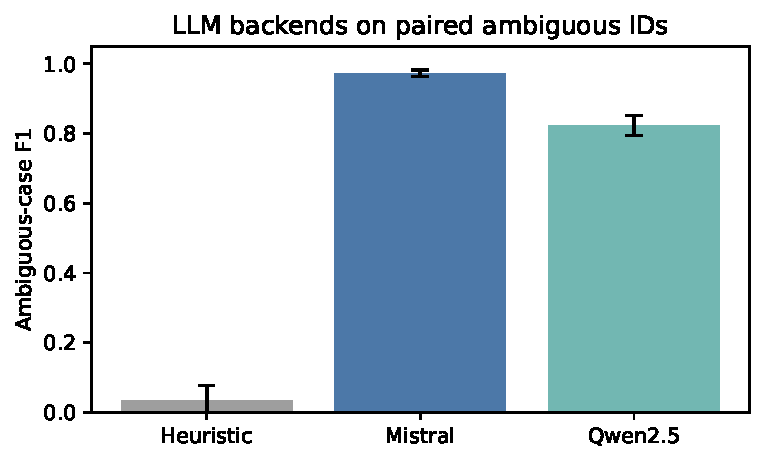
\includegraphics[width=0.85\linewidth]{figures/llm_backends.pdf}
\caption{Mean$\pm$std ambiguous-case F1 across five folds for heuristic, Mistral, and Qwen2.5 backends.}
\label{fig:llm}
\end{figure}

\begin{table}[!t]
\centering
\caption{Paired LLM backend comparison on shared ambiguous case IDs (up to 150 cases/fold).}
\label{tab:llm}
\begin{tabular}{cccc}
\toprule
Fold & Heuristic F1 & Mistral F1 & Qwen2.5 F1 \\
\midrule
0 & 0.042 & 0.959 & 0.807 \\
1 & 0.105 & 0.977 & 0.874 \\
2 & 0.000 & 0.975 & 0.819 \\
3 & 0.021 & 0.984 & 0.802 \\
4 & 0.000 & 0.966 & 0.813 \\
\midrule
Mean & 0.034 & \textbf{0.972} & 0.823 \\
\bottomrule
\end{tabular}
\end{table}


\subsection{Negative Studies: Label-Flip Actor--Critic}
\label{sec:negative}
Allowing a Critic to flip fall$\rightarrow$ADL labels is unsafe under FN-heavy cost. Table~\ref{tab:negative} shows FN exploding (e.g., Fold~0: $6\rightarrow 105$) and recall collapsing from $0.986$ to $0.755$. We therefore (i)~freeze fall/ADL labels in the primary stack, (ii)~restrict critique to action downgrades and rationale grounding (Table~\ref{tab:grounding}), and (iii)~prefer contrastive hard negatives over unconstrained vetoes. Not every ``agent'' addition helps.

\begin{table}[!t]
\centering
\caption{Negative ablation: naive label-flip Actor--Critic (\texttt{gate\_knn\_llm\_actor\_critic}) vs.\ primary stack. The Critic may veto fall predictions, inducing catastrophic FN spikes. Contrastive action critique (labels frozen) is the safe alternative (Table~\ref{tab:grounding}).}
\label{tab:negative}
\begin{tabular}{c ccc ccc c}
\toprule
Fold & \multicolumn{3}{c}{gate\_knn\_llm} & \multicolumn{3}{c}{+Actor--Critic (harmful)} & $\Delta$FN \\
\cmidrule(lr){2-4}\cmidrule(lr){5-7}
 & F1 & Rec. & FN & F1 & Rec. & FN & \\
\midrule
0 & 0.893 & 0.986 & 6 & 0.768 & 0.755 & 105 & +99 \\
1 & 0.851 & 0.911 & 39 & 0.744 & 0.714 & 125 & +86 \\
2 & 0.896 & 0.986 & 6 & 0.757 & 0.725 & 119 & +113 \\
3 & 0.917 & 0.993 & 3 & 0.766 & 0.721 & 122 & +119 \\
4 & 0.898 & 0.981 & 8 & 0.769 & 0.744 & 110 & +102 \\
\midrule
Mean & --- & --- & 12.4 & --- & --- & 116.2 & +103.8 \\
\bottomrule
\end{tabular}
\end{table}


\subsection{Backbone Context}
Table~\ref{tab:backbone} reports detector-only Fold~0 metrics for the backbone zoo. We fix \texttt{cnn\_lstm\_attn} for all agentic tables so comparisons stay fair to the Bhatti-style architecture.

\begin{table}[!t]
\centering
\caption{Tier-1 backbone zoo on Fold~0 (detector-only metrics). Primary paper backbone is \texttt{cnn\_lstm\_attn} (Bhatti-style).}
\label{tab:backbone}
\begin{tabular}{lcccc}
\toprule
Model & F1 & Recall & Spec. & Params \\
\midrule
cnn1d & 0.721 & 0.985 & 0.277 & 43,330 \\
lstm & 0.700 & 0.986 & 0.197 & 201,986 \\
cnn\_lstm & 0.694 & 0.995 & 0.155 & 86,914 \\
\textbf{cnn\_lstm\_attn} & 0.710 & 0.996 & 0.216 & 564,930 \\
tcn & 0.727 & 0.988 & 0.295 & 89,282 \\
modern\_tcn & 0.737 & 0.990 & 0.326 & 30,314 \\
tsmixer & 0.695 & 0.984 & 0.181 & 224,562 \\
patchtst & 0.669 & 0.996 & 0.051 & 150,786 \\
transformer & 0.678 & 0.994 & 0.092 & 158,722 \\
\bottomrule
\end{tabular}
\end{table}


\subsection{Latency and Budget Sensitivity}
Fig.~\ref{fig:latency} and Table~\ref{tab:latency} contrast Tier-1 latency (milliseconds) with the escalated Ollama path (seconds; typically $10$--$14$\,s per escalated window on our Mistral setup). Mean stack latency is lower than the pure escalated path because only ambiguous windows escalate, but the system is a caregiver-facing safety layer, not millisecond impact protection. Fig.~\ref{fig:budget} compares $n{=}1000$ versus archived $n{=}4000$: directional gains hold, so the main budget is not a cherry-picked regime.

\begin{figure}[!t]
\centering
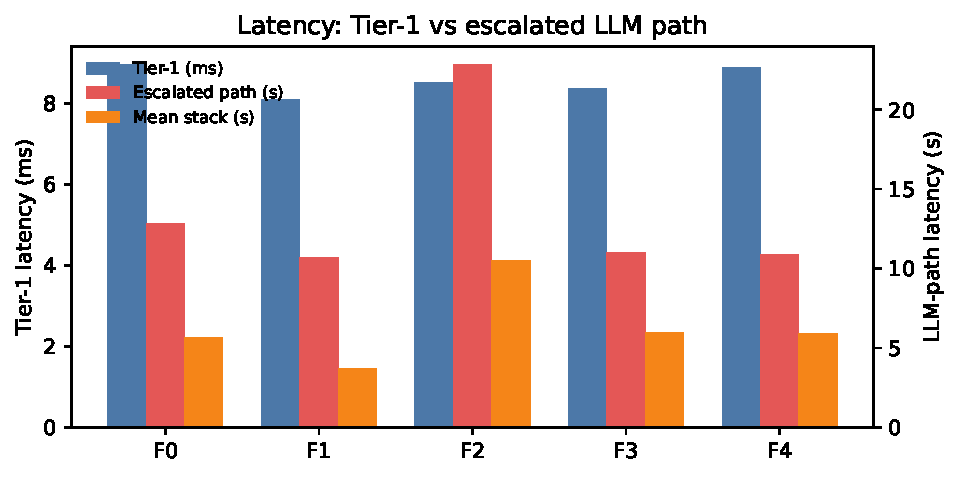
\includegraphics[width=\linewidth]{figures/latency_bars.pdf}
\caption{Latency by fold: Tier-1 (ms, left axis) versus escalated LLM path and mean stack latency (seconds, right axis).}
\label{fig:latency}
\end{figure}

\begin{figure}[!t]
\centering
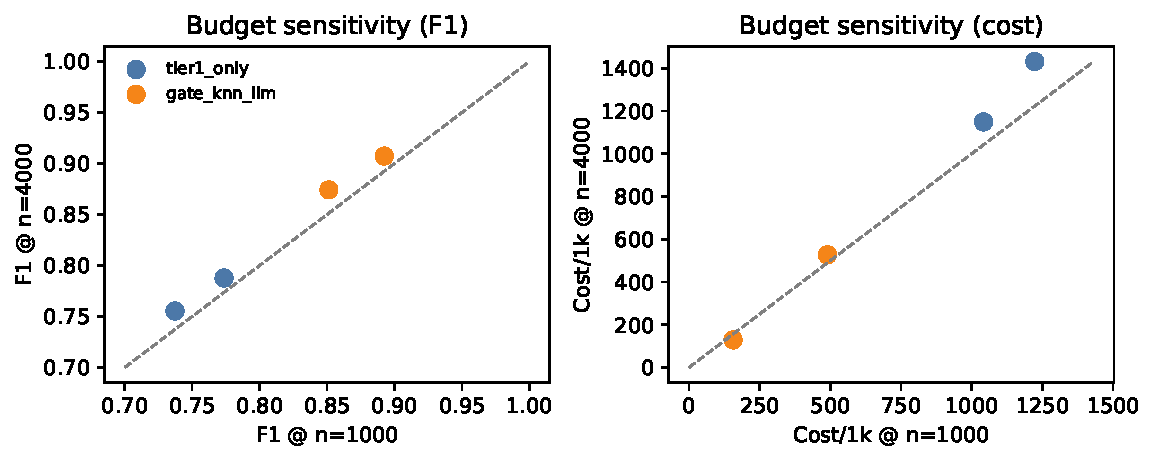
\includegraphics[width=\linewidth]{figures/budget_sensitivity.pdf}
\caption{Budget sensitivity: metrics at $n{=}1000$ versus $n{=}4000$ for Tier-1 and full stack on archived folds.}
\label{fig:budget}
\end{figure}

\begin{table}[!t]
\centering
\caption{End-to-end latency from Ollama agentic runs ($n{=}1000$/fold). Escalated-path latency is dominated by local LLM inference.}
\label{tab:latency}
\begin{tabular}{crrr}
\toprule
Fold & Tier-1 (ms) & Escalated (s) & Mean stack (s) \\
\midrule
0 & 8.96 & 12.81 & 5.68 \\
1 & 8.09 & 10.66 & 3.73 \\
2 & 8.52 & 22.85 & 10.52 \\
3 & 8.36 & 11.00 & 5.99 \\
4 & 8.89 & 10.86 & 5.93 \\
\midrule
Mean & 8.56 & 13.63 & 6.37 \\
\bottomrule
\end{tabular}
\end{table}


\subsection{External Validation on KFall}
\label{sec:kfall}
Beyond Falls reports strong multi-class multi-phase numbers on KFall and notes residual sit/stand confusion. We evaluate our safety layer under a locked binary Fall/ADL protocol matching SisFall costs and folds. Table~\ref{tab:bhattigaps} maps their open gaps to our agents. Tables~\ref{tab:kfallperfold}--\ref{tab:kfallmean} show Tier-1 F1 $0.987{\pm}0.005$ versus stack $0.990{\pm}0.004$ ($\Delta\text{F1}{=}+0.003$) with cost/1000 $50{\rightarrow}26$---stability, not a breakthrough. Fold~0 ablations and LLM pairs appear in Tables~\ref{tab:kfallablation}--\ref{tab:kfallllm}. A 36-class Tier-1 context run (Table~\ref{tab:kfallmc}; macro-F1 $0.541$) is explicitly not a multi-class leaderboard claim.

\begin{table*}[!t]
\centering
\caption{Bhatti \textit{et al.}~2025 limitations versus our multi-agent answers (complementary Q1 claim).}
\label{tab:bhattigaps}
\begin{tabular}{p{0.42\linewidth}p{0.48\linewidth}}
\toprule
Bhatti \textit{et al.} gap & Our multi-agent response \\
\midrule
Softmax force-labels every window; D18/D19 sit/stand confusion & Dual-threshold \textbf{Confidence Gate} escalates ambiguous band \\
Explainability limited to attention weights & Biomechanical \textbf{evidence} + LLM chain-of-thought JSON \\
No retrieval / case memory & MiniLM $k$-NN \textbf{Memory} agent \\
Detection only; no clinical response policy & Cost-sensitive \textbf{Action Agent} ($10\cdot\mathrm{FN}+1\cdot\mathrm{FP}$) \\
Published focus: 36-class multi-phase F1~$\approx$98\%, $\sim$20\,ms & Fair claim: same Tier-1 + agents improve recall/cost under uncertainty (SisFall+KFall) \\
\bottomrule
\end{tabular}
\end{table*}

\begin{table*}[!t]
\centering
\caption{KFall binary external validation: Tier-1 vs.\ full agentic stack ($n{=}1000$/fold, subject-independent). Cost normalized per 1000 windows.}
\label{tab:kfallperfold}
\begin{tabular}{c ccc ccc c}
\toprule
Fold & \multicolumn{3}{c}{Tier-1} & \multicolumn{3}{c}{gate\_knn\_llm} & $\Delta$F1 \\
\cmidrule(lr){2-4}\cmidrule(lr){5-7}
 & F1 & Rec. & Cost/1k & F1 & Rec. & Cost/1k & \\
\midrule
0 & 0.992 & 0.998 & 17 & 0.993 & 1.000 & 7 & +0.001 \\
1 & 0.987 & 0.996 & 31 & 0.986 & 0.996 & 32 & -0.001 \\
2 & 0.987 & 0.994 & 40 & 0.989 & 0.996 & 29 & +0.002 \\
3 & 0.992 & 0.990 & 53 & 0.995 & 0.996 & 23 & +0.003 \\
4 & 0.980 & 0.979 & 109 & 0.989 & 0.994 & 38 & +0.008 \\
\bottomrule
\end{tabular}
\end{table*}

\begin{table}[!t]
\centering
\caption{KFall five-fold mean$\pm$std (binary Fall/ADL). Paired deltas are stack$-$Tier-1.}
\label{tab:kfallmean}
\begin{tabular}{lccc}
\toprule
Mode & F1 & Recall & Cost/1000 \\
\midrule
tier1\_only & 0.987$\pm$0.005 & 0.991$\pm$0.007 & 50$\pm$35 \\
\textbf{gate\_knn\_llm} & \textbf{0.990$\pm$0.004} & \textbf{0.996$\pm$0.002} & \textbf{26$\pm$12} \\
\midrule
\multicolumn{4}{l}{\textit{Paired $\Delta$ (bootstrap 95\% CI)}} \\
f1 & +0.003 & [0.000, 0.006] & $p$=0.1250 \\
recall & +0.005 & [0.001, 0.010] & $p$=0.0679 \\
cost\_per\_1000 & -24.200 & [-48.400, -5.800] & $p$=0.1250 \\
\bottomrule
\end{tabular}
\end{table}

\begin{table}[!t]
\centering
\caption{KFall Fold~0 ablation ladder ($n{=}1000$). Full stack requires $k$-NN+LLM.}
\label{tab:kfallablation}
\begin{tabular}{lcccc}
\toprule
Mode & F1 & Recall & Cost & Esc.\ F1 \\
\midrule
tier1\_only & 0.992 & 0.998 & 17 & 0.000 \\
gate\_only & 0.992 & 0.998 & 17 & 0.750 \\
gate\_knn & 0.991 & 0.994 & 36 & 0.400 \\
gate\_llm & 0.976 & 0.998 & 33 & 0.250 \\
\textbf{gate\_knn\_llm} & 0.993 & 1.000 & 7 & 0.889 \\
\bottomrule
\end{tabular}
\end{table}

\begin{table}[!t]
\centering
\caption{KFall paired LLM backends on shared ambiguous IDs.}
\label{tab:kfallllm}
\begin{tabular}{cccc}
\toprule
Fold & Heuristic F1 & Mistral F1 & Qwen F1 \\
\midrule
0 & 0.167 & 0.880 & 0.500 \\
1 & 0.000 & 1.000 & 0.364 \\
2 & 0.000 & 1.000 & 0.600 \\
3 & 0.000 & 0.571 & 0.250 \\
4 & 0.273 & 0.974 & 0.809 \\
\midrule
Mean & 0.088 & \textbf{0.885} & 0.504 \\
\bottomrule
\end{tabular}
\end{table}

\begin{table}[!t]
\centering
\caption{Context-only 36-class Tier-1 on KFall transition (Fold~0). Not a claim against Bhatti's published multi-class table.}
\label{tab:kfallmc}
\begin{tabular}{lccc}
\toprule
Setting & Acc. & Macro-F1 & Weighted-F1 \\
\midrule
Our Tier-1 (transition, fold0) & 0.585 & 0.541 & 0.583 \\
Bhatti \textit{et al.} (published, multi-phase) & --- & $\approx$0.98 & --- \\
\bottomrule
\end{tabular}
\end{table}


\section{Discussion}
\label{sec:discussion}

\subsection{What Changes Relative to Detection-Only Work}
Fair numerical comparison here is \texttt{tier1\_only} versus \texttt{gate\_knn\_llm} under identical SisFall folds and checkpoints (Table~\ref{tab:positioning}). SisFall is our primary runnable binary+near-fall corpus with D18/D19 instrumentation; KFall multi-class multi-phase remains Bhatti's native setting.

\subsection{Where the Gains Come From}
Outperformance is threefold: higher F1 and recall on every main fold; large reduction in FN-weighted cost; high escalated-subset F1 when the gate defers. Ablations show retrieval and LLM reasoning interact---neither alone reproduces the headline stack. Near-fall FAR improvements are modest and are not sold as the primary differentiator.

\subsection{Statistics, Seeds, and Robustness}
Table~\ref{tab:stats} reports paired $\Delta$ statistics with BCa CIs and $5/5$ directional consistency. Multi-seed Fold~0 Ollama sweeps (Table~\ref{tab:seeds}) give stack F1 $0.905{\pm}0.005$ across seeds $\{42,43,44\}$.

\subsection{Split-Conformal Gating and Duty-Cycle Trade-offs}
\label{sec:conformal}
We implement a binary split-conformal gate with nonconformity $s=1-\hat{p}(y)$ and quantile $\hat{q}$~\cite{vovk2005algorithmic,angelopoulos2023gentle}. Singleton sets route at the edge; doubleton sets escalate. At $\alpha{=}0.05$ (Table~\ref{tab:conformalgate}), edge FN stays near or below the nominal level on folds~0--3 while escalation rises ($0.58$--$0.83$) relative to the cost gate ($0.38$--$0.47$). Fold~4 exceeds $\alpha$ on edge FN ($0.087$) and is reported honestly. Table~\ref{tab:pareto} summarizes duty-cycle Pareto points trading clinical cost against escalation. Table~\ref{tab:partitionfallback} reports the offline Bayes threshold~\eqref{eq:tau_star} with zero escalation (high recall, elevated FP). Table~\ref{tab:robustness} shows Tier-1 routing F1 under $\pm 10^\circ$/$\pm 15^\circ$ orientation perturbation and $50$/$100$\,Hz resampling: clean $0.768{\pm}0.017$ versus $0.754{\pm}0.023$ at $\pm 15^\circ$. Table~\ref{tab:knnk} shows $k\in\{1,5,10\}$ is flat under a heuristic LLM on the main protocol---retrieval width alone does not move that backend.

\begin{table}[!t]
\centering
\caption{Split conformal gate audit ($\alpha{=}0.05$): edge-decision FN rate vs.\ cost-calibrated gate escalation.}
\label{tab:conformalgate}
\begin{tabular}{c ccc ccc}
\toprule
Fold & $q_{\hat{}}$ & Esc.\ (conf.) & Edge FN & F1 (conf.) & Esc.\ (cost) & F1 (cost) \\
\midrule
0 & 0.830 & 0.58 & 0.0166 & 0.774 & 0.38 & 0.774 \\
1 & 0.926 & 0.83 & 0.0301 & 0.737 & 0.47 & 0.737 \\
2 & 0.904 & 0.70 & 0.0166 & 0.764 & 0.40 & 0.764 \\
3 & 0.856 & 0.61 & 0.0104 & 0.787 & 0.38 & 0.787 \\
4 & 0.630 & 0.17 & 0.0874 & 0.778 & 0.22 & 0.778 \\
\bottomrule
\end{tabular}
\end{table}

\begin{table}[!t]
\centering
\caption{Duty-cycle Pareto operating points (tier-1 routing, pooled folds): clinical cost vs.\ escalation.}
\label{tab:pareto}
\begin{tabular}{ccccc}
\toprule
Point & $\tau_{\mathrm{low}}$ & $\tau_{\mathrm{high}}$ & Esc.\ rate & Cost \\
\midrule
Min cost & 0.05 & 0.60 & 0.57 & 1015 \\
Q25 esc. & 0.30 & 0.70 & 0.34 & 1015 \\
Q50 esc. & 0.40 & 0.95 & 0.48 & 1042 \\
Q75 esc. & 0.30 & 0.95 & 0.61 & 1223 \\
\bottomrule
\end{tabular}
\end{table}

\begin{table}[!t]
\centering
\caption{Offline partition fallback: single Bayes threshold $\tau^\ast{=}1/(\beta{+}1)$, no escalation ($\beta{=}10$).}
\label{tab:partitionfallback}
\begin{tabular}{lc}
\toprule
Metric & Mean $\pm$ std (5 folds) \\
\midrule
F1 & 0.639 $\pm$ 0.006 \\
Recall & 0.988 $\pm$ 0.008 \\
\bottomrule
\end{tabular}
\end{table}

\begin{table}[!t]
\centering
\caption{Tier-1 routing robustness (cost gate): mean F1 across folds under IMU perturbations.}
\label{tab:robustness}
\begin{tabular}{lc}
\toprule
Condition & Mean F1 \\
\midrule
clean & 0.768 $\pm$ 0.017 \\
resample\_100hz & 0.766 $\pm$ 0.016 \\
resample\_50hz & 0.766 $\pm$ 0.015 \\
rotate\_10deg & 0.763 $\pm$ 0.020 \\
rotate\_15deg & 0.754 $\pm$ 0.023 \\
\bottomrule
\end{tabular}
\end{table}

\begin{table}[!t]
\centering
\caption{$k$-NN retrieval ablation ($k \in \{1,5,10\}$, fold~0, heuristic LLM).}
\label{tab:knnk}
\begin{tabular}{cccc}
\toprule
$k$ & F1 & Recall & Escalation \\
\midrule
1 & 0.384 & 0.240 & 0.38 \\
5 & 0.384 & 0.240 & 0.38 \\
10 & 0.384 & 0.240 & 0.38 \\
\bottomrule
\end{tabular}
\end{table}

\begin{table}[!t]
\centering
\caption{Multi-seed robustness on Fold~0 ($n{=}1000$). Stack backend: Ollama/Mistral.}
\label{tab:seeds}
\begin{tabular}{ccccc}
\toprule
Seed & Tier-1 F1 & Stack F1 & Stack Rec. & Cost/1k \\
\midrule
42 & 0.747 & 0.909 & 0.998 & 95 \\
43 & 0.740 & 0.907 & 0.995 & 105 \\
44 & 0.746 & 0.899 & 1.000 & 96 \\
\midrule
Mean$\pm$std & 0.745$\pm$0.004 & 0.905$\pm$0.005 & --- & --- \\
\bottomrule
\end{tabular}
\end{table}


\subsection{Limitations}
Local LLMs add seconds on escalated windows. Escalation is substantial on SisFall ($\approx 47\%$ main, $\approx 59\%$ ambiguous) and low on binary KFall ($\approx 1.1\%$); we do not claim sub-$5\%$ SisFall duty cycles. KFall $\Delta$F1 is $+0.003$. With five folds, nonparametric $p$-values are coarse; bootstrap CIs carry the uncertainty claim. Action-agent effects are simulated---no live clinical trial. We did not profile battery or embedded energy. Split conformal helps edge-FN audits but can increase escalation versus the cost gate. Free-living unlabeled streams, distilled on-device reasoners, and prospective eldercare validation remain future work.

\section{Conclusion}
\label{sec:concl}

We wrapped a fixed Bhatti-style Tier-1 IMU detector in a confidence-gated multi-agent stack that escalates ambiguous windows to retrieval-augmented LLM reasoning and a cost-sensitive Action Agent. Under a locked SisFall protocol, the full stack improves F1, recall, and FN-weighted response cost on every main fold, with the largest relative recovery on a near-fall stress benchmark. Ablations, LLM pairs, conformal audits, and a negative actor--critic study bound where the gains---and the risks---actually sit. The claim is a software safety layer around a strong detector, not a replacement for backbone-centric fall detection research.

\section*{Acknowledgment}
The authors thank collaborators and computing facility staff for GPU support. Author identities are withheld for double-blind review.

\appendices
\section{Reproducibility Notes}
\label{app:repro}
Artifacts: per-fold JSON under \texttt{results/fold\{0--4\}/}, aggregates \texttt{results/aggregate\_*}, tables under \texttt{tables/}, figures under \texttt{figures/}, and plain-text mirrors under \texttt{results\_text/} (including \texttt{DATA\_LOCK.txt}). Regenerators in the companion code release:
\begin{verbatim}
python scripts/aggregate_folds.py --results-dir results
python scripts/generate_paper_tables.py
python scripts/plot_paper_figures.py
python scripts/run_astar_experiments.py
\end{verbatim}

\section{Homogeneous Protocol Details}
\label{app:protocol}
Locked settings: seed $42$, five subject folds, \texttt{max\_train}${}={}$40000, main \texttt{max\_test}${}={}$1000, LLM compare up to $150$ ambiguous cases/fold, cost weights $\mathrm{FN}{=}10$, $\mathrm{FP}{=}1$, required near-fall codes D18/D19 with minimum $80$ each in capped slices (\texttt{configs/paper\_protocol.yaml}).

\bibliographystyle{IEEEtran}
\bibliography{refs}

\end{document}
